\achapter

\answer $ F _ { \text{min} } = 1 4 4   $公斤力

\answer $ 15 $吨

\answer $ 25 $公斤力
% 382.jpg

\answer $ 10 $米/秒

\answer $ 5.91 $米

\answer (1) $ 50 $公斤

(2) 上升时,$ 75 $公斤;下降时,$ 25 $公斤

\answer (1) $ \left( M - m \right) g  $

(2) $ \left( M - m \right) g - m a   $

\answer (1) $ 98 $厘米/秒

(2) $ 17.6 $牛顿

\answer $ \mu = \dfrac { m _ { B } \left( g - a \right) - m _ { A } a } { m _ { A } g }   $

\answer $ \dfrac { F _2 }{ F _1 } = \dfrac { 1 } { \cos \alpha - \mu \sin \alpha } $


\answer (1) $ 4.0\text{吨力} \approx 39.2 \times 10 ^ 3 \text{牛顿} $

(2) $ 4.0\text{吨力} \approx 39.2 \times 10 ^ 3 \text{牛顿} $

(3) $ 4.0\text{吨力} \approx 39.2 \times 10 ^ 3 \text{牛顿} $

(4) $ 40.8 \times 10 ^ 3 \text{牛顿} \approx 4.1 \times 10 ^ 4 \text{牛顿} $

(5) $ 3.6 \times 10 ^ 4 \text{牛顿} $

(6) $ 2.45 $米/秒

\answer $ m_2 $在桌上时,加速度$  a = 4 . 9   $米/秒\textsuperscript{2},张力$  T = 1 . 4 7   $牛顿;

$ m_1 $在桌上时,加速度$  a = 2 . 4 5   $米/秒,张力$ T=1.47 $牛顿

\answer $ a = \dfrac { m g - \mu \left( m _ { 1 } + m _ { 2 } + m _ { 3 } \right) g } { m + \left( m _ { 1 } + m _ { 2 } + m _ { 3 } \right) }   $

$ T _ { 1 } = m _ { 1 } \left( a + \mu g \right)  $

$ T _ { 2 } = \left( m _ { 1 } + m _ { 2 } \right) \left( a + u g \right)  $

$ T _ { 3 } = m \left( g - a \right) $

\answer $ a = \dfrac { m _ { 1 } \sin \alpha -m _ { 2 } } { m _ { 1 } + m _ { 2 } + m _ { 3 } } g  $

$ T _ { 1 } = m _ { 1 } \left( g \sin \alpha - a \right)   $

$ T _ { 2 } = m _ { 2 } a   $

取$ x $轴向右,$ y $轴向上,则得$ A $点承受之支持力为

$ \vec{N} = \vec{i} N _ { x } + \vec{j} N _ { y }  $

% 383.jpg
$ N _ { x } = T _ { 1 } \cos \alpha   $

$ N _ { y } = T _ { 1 } \sin \alpha + T _ { 2 }  $

$ B $点拉滑轮的绳$ d $承受的张力$  T = \sqrt { 2 } T _ { 2 }  $

\answer $ \mu _ { 0 } = 0 . 5 7 7$ , $\mu = 0 . 5 3 0   $

\answer (1) $ F = \left( M + m \right) g \tg \alpha $

(2) $ a = g \tg \alpha  $

\answer (1) $ m g - \beta v = m a $

\aindent $ m g - \beta \dot{z} = m \ddot{z}  $

(2) $ v \left( t _ { 0 } \right) = \dfrac { m } { \beta } g $

(4)略

\answer (1) $ g \sin \theta $,沿斜面向下

(2) $ g \sin \theta $,沿斜面向下

(3) $ \left( g - a \right) \sin \theta   $,当$  g > a   $时沿斜面向下

\aindent 当$  g < a   $时沿斜面往上

\aindent 当$  g = a   $时物与斜面相对静止

(4) $ \left( g + a \right) \sin \theta   $,沿斜面向下

(5) 0

(6) $ m \left( g - a \right) \cos \theta $

\stepcounter{answer}
\answer $ a _ { 1 } = \dfrac { 3 } { 7 } g $向下

$ a _ { 2 } = \dfrac { 1 } { 7 } g$,向上

$ a _ { 3 } = \dfrac { 1 } { 7 } g $,向上

$ T _ { 1 } = 2 . 2 3   $牛顿

$ T _ { 2 } = - 4 . 4 6   $牛顿

\answer $ a _ { 2 } = 97.4 $米/秒

\answer $ \mu _ { \text{min} } = 0 . 3 9 4  $

\answer 张力$ T = \dfrac { M g } { 2 \uppi } \ctg \dfrac { \alpha } { 2 }  $

% 384.jpg
\answer (1) $ v _ { 0 } = \sqrt { l g } = 1 9 8  $ 厘米/秒

(2) $ T = 3 m g = 2 . 9 4$牛顿

\answer (1) $v=\sin \theta \sqrt{\dfrac{l g}{\cos \theta}}=\sqrt{g l \tg \theta \sin \theta}$

\makebox[1.5em]{}$ F = m g \tg \theta   $

\answer $ h = R - \dfrac{ g }{\omega ^ 2} $ ,或在碗底不动

\answer (1) $ v = \sqrt { g h } $

(2) $\sqrt{g h \dfrac{1-\mu \operatorname{tg} \theta / 2}{1+\mu c \operatorname{tg} \theta / 2}} \leqslant v \leqslant \sqrt{g h \dfrac{1+\mu \operatorname{tg} \theta / 2}{1-\mu \operatorname{ctg} \theta / 2}}$

\answer $\sqrt{R g \dfrac{\sin \alpha-\mu \cos \alpha}{\cos \alpha+\mu \sin \alpha}} \leqslant v \leqslant \sqrt{R g \dfrac{\sin \alpha+\mu \cos \alpha}{\cos \alpha-\mu \sin \alpha}}$

若$  v < \sqrt{R g \dfrac{\sin \alpha-\mu \cos \alpha}{\cos \alpha+\mu \sin \alpha}}   $,则车往里倒或下滑

若$  v > \sqrt{R g \dfrac{\sin \alpha+\mu \cos \alpha}{\cos \alpha-\mu \sin \alpha}} $,则车往外倒或往外跑

若$ \mu = 1 $且$  \theta = \uppi / 4   $,则任何速率都可安全行驶

\answer (1) $ \dfrac { W } { 2 \cos \theta } $

(2) $ \dfrac { W } { 2 } \tg \theta  $

\answer (1) $ T \left( \theta \right) = \lambda R g \sin \theta  $

(2) $ N \left( \theta \right) \Delta \theta = 2 \lambda R g \sin \alpha \cdot \Delta \theta  $
\begin{figurex}
    \centering
    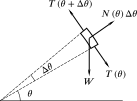
\includegraphics{figure/figa03.01}
    \caption{}
    \label{figa:03.01}
\end{figurex}

$\sum N _ {\text{水平}} = \displaystyle \int_{0}^{\frac{\pi}{2}} N(\theta) \cos \theta d \theta=\lambda P g=T\left(\dfrac{\pi}{2}\right)=T_{A}$\\
这是绳的平衡条件

\answer (1) $ a = \dfrac y L { g }   $\vspace{-0.5em}

(2) $ y \left( t \right) = y _ { 0 } \ch \sqrt { \dfrac g L }  t $

\answer $ T = M \omega ^ { 2 } l \big/ \left( 2 \uppi \right) ^ { 2 }   $

\answer (1) \vspace{-2em}
\begin{figurex}
    \centering
    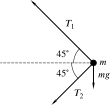
\includegraphics{figure/figa03.02}
    \caption{}
    \label{figa:03.02}
\end{figurex}

(2) $ T _ { 1 } = \dfrac { 1 } { 2 } \left( m \omega ^ { 2 } l + \sqrt { 2 } m g \right) $

\aindent $ T _ { 2 } = \dfrac { 1 } { 2 } \left( m \omega ^ { 2 } l - \sqrt { 2 } m g \right) $

\answer $ T _ { A } \big/ T _ { B } = e ^ { - \mu \theta }  $

\answer (1) 图略

(2) $\begin{cases}T-m_{1} g=m_{1} a \\ m_{2} g \sin \theta-T=m_{2} a \\ N-m_{2} g \cos \theta=0\end{cases}$

\aindent $T=\dfrac{m_{1} m_{2} g(1+\sin \theta)}{m_{1}+m_{2}}$

\aindent $a=\dfrac{\left(m_{2} \sin \theta-m_{1}\right) g}{m_{1}+m_{2}}$

(3) $\mu_{\text { min }}=\dfrac{\cos \theta\left(m_{2} \sin \theta-m_{1}\right)}{m_{1}(1+\sin \theta)^{2}+\left(m_{1}+m_{2}\right)\left(M \operatorname{/} m_{2}+\cos ^{2} \theta\right)}$

% 386.jpg
\answer $\Bigl(\dfrac{\sin \theta-\mu \cos \theta}{\mu \sin \theta+\cos \theta}\Bigr) g \leqslant a \leqslant\Bigl(\dfrac{\sin \theta+\mu \cos \theta}{\cos \theta-\mu \sin \theta}\Bigr) g$

\answer 拱形、桥受压力 $ N = m g \cos \theta - m  v ^ { 2 }  \operatorname{/}  R    $

凹形,桥受压力$  N = m g \cos \theta + m v ^ { 2 } \operatorname{/} R $
